\documentclass[12pt]{beamer}
\usepackage{../Estilos/BeamerMAF}
\usepackage{../Estilos/ColoresLatex}
%Sección para el tema de beamer, con el theme, usercolortheme y sección de footers
\usetheme{Frankfurt}
\usecolortheme{beaver}
%\useoutertheme{default}
\setbeamercovered{invisible}
% or whatever (possibly just delete it)
\setbeamertemplate{section in toc}[sections numbered]
\setbeamertemplate{subsection in toc}[subsections numbered]
\setbeamertemplate{subsection in toc}{\leavevmode\leftskip=3.2em\rlap{\hskip-2em\inserttocsectionnumber.\inserttocsubsectionnumber}\inserttocsubsection\par}
% \setbeamercolor{section in toc}{fg=blue}
% \setbeamercolor{subsection in toc}{fg=blue}
% \setbeamercolor{frametitle}{fg=blue}
\setbeamertemplate{caption}[numbered]

\setbeamertemplate{footline}
\beamertemplatenavigationsymbolsempty
\setbeamertemplate{headline}{}


\makeatletter
% \setbeamercolor{section in foot}{bg=gray!30, fg=black!90!orange}
% \setbeamercolor{subsection in foot}{bg=blue!30!yellow, fg=red}
% \setbeamercolor{date in foot}{bg=black, fg=white}
\setbeamertemplate{footline}
{
  \leavevmode%
  \hbox{%
  \begin{beamercolorbox}[wd=.333333\paperwidth,ht=2.25ex,dp=1ex,center]{section in foot}%
    \usebeamerfont{section in foot} \insertsection
  \end{beamercolorbox}%
  \begin{beamercolorbox}[wd=.333333\paperwidth,ht=2.25ex,dp=1ex,center]{subsection in foot}%
    \usebeamerfont{subsection in foot}  \insertsubsection
  \end{beamercolorbox}%
  \begin{beamercolorbox}[wd=.333333\paperwidth,ht=2.25ex,dp=1ex,right]{date in head/foot}%
    \usebeamerfont{date in head/foot} \insertshortdate{} \hspace*{2em}
    \insertframenumber{} / \inserttotalframenumber \hspace*{2ex} 
  \end{beamercolorbox}}%
  \vskip0pt%
}







\setbeamercolor{section in foot}{bg=deepcarmine, fg=white}
\setbeamercolor{subsection in foot}{bg=flame, fg=white}
\setbeamercolor{date in foot}{bg=blue, fg=white}

\makeatletter
\setbeamertemplate{footline}
{
\leavevmode%
\hbox{%
\begin{beamercolorbox}[wd=.333333\paperwidth,ht=2.25ex,dp=1ex,center]{section in foot}%
  \usebeamerfont{section in foot} \insertsection
\end{beamercolorbox}%
\begin{beamercolorbox}[wd=.333333\paperwidth,ht=2.25ex,dp=1ex,center]{subsection in foot}%
  \usebeamerfont{subsection in foot}  \insertsubsection
\end{beamercolorbox}%
\begin{beamercolorbox}[wd=.333333\paperwidth,ht=2.25ex,dp=1ex,right]{date in head/foot}%
  \usebeamerfont{date in head/foot} \insertshortdate{} \hspace*{1.5em}
  \insertframenumber{} / \inserttotalframenumber \hspace*{2ex} 
\end{beamercolorbox}}%
\vskip0pt%
}
\makeatother
\usefonttheme{serif}
\setbeamercolor{frametitle}{bg=lavenderblue}
\resetcounteronoverlays{saveenumi}

\date{}

\title{\large{Tema 5 - El átomo de hidrógeno}}
\subtitle{Funciones Especiales }
\author{M. en C. Gustavo Contreras Mayén}

\begin{document}
\maketitle
\fontsize{14}{14}\selectfont
\spanishdecimal{.}

\section*{Contenido}
\frame[allowframebreaks]{\tableofcontents[currentsection, hideallsubsections]}

\section{Partícula en un potencial central}
\frame{\tableofcontents[currentsection, hideothersubsections]}
\subsection{Ecuación de Schrödinger}

%Ref. Schaum's (1998) Quantum mechanics.

\begin{frame}
\frametitle{Definiendo el problema}
El Hamiltoniano de una partícula de masa $M$ dentro de un potencial central $V (r)$ es:
\pause
\begin{align}
H = \dfrac{\vb{p}^{2}}{2 M} + V (r) = - \dfrac{\hbar^{2}}{2 M} \, \laplacian + V (r)
\label{eq:ecuacion_08_01}
\end{align}
\end{frame}
\begin{frame}
\frametitle{El Laplaciano}
Donde el operador Laplaciano $\laplacian$ en coordenadas esféricas es:
\pause
\begin{eqnarray}
\begin{aligned}[b]
\laplacian = \dfrac{1}{r} \pdv[2]{r} &+ \dfrac{1}{r^{2}} \bigg[ \pdv[2]{\theta} + \dfrac{1}{\sin \theta} \, \pdv{\theta} + \\[0.5em]
\dfrac{1}{\sin^{2} \theta} \, \pdv[2]{\phi} \bigg]
\end{aligned}
\label{eq:ecuacion_08_02}
\end{eqnarray}
\end{frame}
\begin{frame}
\frametitle{El momento angular}
Considerando que el momento angular se puede expresar como:
\pause
\begin{eqnarray}
\begin{aligned}
\hat{L}_{x} &= - i \, \hbar \, \left( y \, \pdv{z} - z \, \pdv{y} \right) \\[0.5em] \pause
\hat{L}_{y} &= - i \, \hbar \, \left( z \, \pdv{x} - x \, \pdv{z} \right) \\[0.5em] \pause
\hat{L}_{z} &= - i \, \hbar \, \left( x \, \pdv{y} - y \, \pdv{x} \right)
\end{aligned}
\label{eq:ecuacion_01_03a}
\end{eqnarray}
\end{frame}
\begin{frame}
\frametitle{Reescribiendo el Hamiltoniano}
Entonces podemos escribir el Hamiltoniano $H$ como:
\pause
\begin{align}
H = - \dfrac{\hbar^{2}}{2 M} \, \dfrac{1}{r} \, \pdv[2]{r} + \dfrac{1}{2 M r^{2}} \, \vb{L}^{2} + V (r)
\label{eq:ecuacion_08_03}
\end{align}
\end{frame}

%Las tres componentes del operador $\vb{L}$ conmutan con $\vb{L}^{2}$, y



% El potencial en el átomo de hidrógeno es el potencial de interacción de tipo Coulomb entre el núcleo y el electrón.
% \par
% Este es un potencial radial, es decir, depende solamente de la distancia al núcleo $(r)$:
% \begin{align}
% V = V(r) = - \dfrac{k \, Z \, e^{2}}{r}
% \label{eq:ecuacion_01}
% \end{align}
% donde $Z$ el número atómico (en este caso $Z=1$), $e$ es la carga del electrón y $k$ es la constante de Coulomb.
% \par
% Por lo tanto el Hamiltoniano cuántico (el operador correspondiente a la energía total de sistema) se escribe como:
% \begin{align}
% H = - \dfrac{\hbar^{2}}{2 \, m} \, \laplacian + V(r)
% \label{eq:ecuacion_02} 
% \end{align}

% El sistema de coordenadas esféricas es el más adecuado para el problema: la ecuación de Schrödinger será más fácil de resolver en este sistema.
% \par
% Como ya sabemos expresar el Laplaciano en este sistema, haremos uso de esa expresión:
% \begin{align*}
% \laplacian = \dfrac{1}{r^{2}} \pdv{r} \left( r^{2} \pdv{\phi}{r} \right) {+} \dfrac{1}{r^{2} \sin \theta} \pdv{\theta} \left( \sin \theta \pdv{\phi}{\theta} \right) {+} \dfrac{1}{r^{2} \sin^{2} \theta} \pdv[2]{\phi}{\phi} 
% \end{align*}
% La expresión para el Laplaciano es complicada así que buscaremos una expresión más adecuada para resolver la ecuación de Schrödinger más fácilmente.

% \subsection{Momento angular.}

% La teoría del momento angular en mecánica cuántica es de gran importancia tanto por el número como por la variedad de sus consecuencias.
% \par
% A partir de la espectroscopía rotacional, que depende del momento angular de las moléculas, se consigue información acerca de las dimensiones y formas de moléculas.
% \par
% Utilizando los espectros de resonancia magnética nuclear y de resonancia paramagnética electrónica, cuyo origen es el momento angular de espín de núcleos y electrones, se consigue información sobre la estructura y configuración de moléculas.
% \par
% El momento angular orbital de los electrones en los átomos define las forma de los orbitales atómicos los cuales, a su vez, determinan la orientación de los enlaces y la estereoquímica de las moléculas. El momento angular de un sistema es muy importante, cuando \emph{es una constante de movimiento}, es decir, cuando se conserva, porque en este caso sirve para clasificar los niveles de energía del sistema.
% \par
% En mecánica cuántica los operadores de momento angular orbital son:
% \begin{align}
% \begin{aligned}
% \hat{L}_{x} &=& - i \, \hbar \, \left( y \, \pdv{z} - z \, \pdv{y} \right) \\[0.5em] 
% \hat{L}_{y} &=& - i \, \hbar \, \left( z \, \pdv{x} - x \, \pdv{z} \right) \\[0.5em] 
% \hat{L}_{z} &=& - i \, \hbar \, \left( x \, \pdv{y} - y \, \pdv{x} \right)
% \end{aligned}
% \label{eq:ecuacion_01_03a}
% \end{align}

% El cuadrado del operador momento angular es tal que:
% \begin{align}
% \hat{L}^{2} = \hat{L} \cdot \hat{L} = \hat{L}_{x}^{2} + \hat{L}_{y}^{2} + \hat{L}_{z}^{2}
% \label{eq:ecuacion_01_03b}
% \end{align}

% Para aplicar estos operadores sobre funciones del tipo $\psi(r, \theta, \phi)$ es necesario expresarlos en coordenadas polares. Utilizando las relaciones:
% \begin{align*}
% r^{2} &= x^{2} + y^{2} +z^{2} \\
% \cos \theta &= \dfrac{z}{\sqrt{x^{2} + y^{2} +z^{2}}} \\
% \tan \phi &= \dfrac{y}{x}
% \end{align*}
 
% Para luego aplicar las derivadas parciales $\pdv*{x}$, $\pdv*{y}$ y $\pdv*{z}$, se tiene:
% \begin{align}
% \begin{aligned}
% \hat{L}_{x} &= + i\, \hbar \, \left( \sin \phi \,\pdv{\theta} + \cot \theta\, \cos \phi \, \pdv{\phi} \right) \\[0.5em] 
% \hat{L}_{y} &= - i\, \hbar \, \left( \cos \phi \,\pdv{\theta} - \cot \theta\, \sin \phi \, \pdv{\phi} \right) \\[0.5em] 
% \hat{L}_{z} &= - i\, \hbar \, \pdv{\phi}
% \end{aligned}
% \label{eq:ecuacion_01_04a}
% \end{align}

% El cuadrado del operador momento angular es:
% \begin{align}
% \hat{L}^{2} = - \hbar^{2} \left( \dfrac{1}{\sin \theta} \pdv{\theta} \, \sin \theta \, \pdv{\theta} + \dfrac{1}{\sin^{2} \theta} \, \pdv[2]{\phi} \right)
% \label{eq:ecuacion_01_04b}
% \end{align}

% Es importante notar que solo se utiliza el operador $\hat{L}^{2}$ o sus componentes, pero nunca el operador $\hat{L}$ directamente, ya que el momento angular es un vector $\va{L}$ y no un escalar.

% \subsection{Constante de movimiento.}

% La condición para que el operador $\hat{O}$ represente una \emph{constante de movimiento} de un sistema es que se cumpla la relación:
% \begin{align}
% \hat{O} \, \hat{H} = \hat{H} \, \hat{O}
% \label{eq:ecuacion_01_05}
% \end{align}
% donde $\hat{H}$ es el Hamiltoniano del sistema.
% \par
% La relación anterior implica que el conmutador:
% \begin{align}
% [\hat{O}, \hat{H}] = \hat{O} \hat{H} - \hat{H} \, \hat{O}
% \label{eq:ecuacion_01_06}
% \end{align}
% vale cero.
% \par
% En efecto, cuando dos operadores conmutan, existe un conjunto de funciones que son funciones propias de los dos operadores simultáneamente. Es decir, que la misma función $\psi$ que caracteriza el estado del sistema con energía $E$:
% \begin{align*}
% \hat{H} \, \psi = E \, \psi
% \end{align*}
% también caracteriza el estado del sistema con propiedad $\hat{O}$ igual a $0$:
% \begin{align*}
% \hat{O} \, \psi = 0 \, \psi
% \end{align*}

% Dicho de otra manera, cuando el sistema se encuentra en el estado caracterizado por $\psi$, su energía es $E$ y su propiedad $\hat{O}$ es $o$. Ambos valores $E$ y $o$ son constantes mientras el sistema permanezca en el mismo estado $\psi$.
% \par
% En los casos en los que $\psi$ sea degenerada, siempre será posible construir una combinación lineal de las funciones propias correspondientes a $E$ tal que sea también función propia de $\hat{O}$.

\subsection{Reglas de conmutación}

\begin{frame}
\frametitle{Conmutación entre operadores}
Las reglas de conmutación entre los operadores de momento angular y sus componentes pueden ser deducidas fácilmente utilizando las expresiones en coordenadas cartesianas y algunas identidades de los conmutadores como:
\pause
\begin{eqnarray*}
\begin{aligned}
\comm{\hat{A} + \hat{B}}{\hat{C}} &= \pause \comm{\hat{A}}{\hat{C}} + \comm{\hat{B}}{\hat{C}} \\[0.5em] \pause
\comm{\hat{A}^{2}}{\hat{B}} &= \pause \comm{\hat{A}}{\hat{B}} \, \hat{A} + \hat{A} \, \comm{\hat{A}}{\hat{B}}
\end{aligned}
\end{eqnarray*}
\end{frame}
\begin{frame}
\frametitle{Conmutación entre componentes del momento}
Se cumple entonces que:
\pause
\begin{eqnarray}
\begin{aligned}
\comm{L_{x}}{L_{y}} &= i \, \hbar \, L_{z} \\[0.5em] \pause
\comm{L_{y}}{L_{z}} &= i \, \hbar \, L_{x} \\[0.5em] \pause
\comm{L_{z}}{L_{x}} &= i \, \hbar \, L_{y} \\[0.5em] \pause
\comm{\vb{L}^{2}}{L_{x}} = \comm{\vb{L}^{2}}{L_{y}} &= \comm{\vb{L}^{2}}{L_{z}} = 0
\end{aligned}
\label{eq:ecuacion_01_07}
\end{eqnarray}
\end{frame}
\begin{frame}
\frametitle{Resultado de la conmutación}
Entonces: \pause
\setbeamercolor{item projected}{bg=lava,fg=white}
\setbeamertemplate{enumerate items}{%
\usebeamercolor[bg]{item projected}%
\raisebox{1.5pt}{\colorbox{bg}{\color{fg}\footnotesize\insertenumlabel}}%
}
\begin{enumerate}[<+->]
\item $\vb{L}^{2}$ conmuta con cualquiera de sus componentes.
\item Pero las componentes no conmutan entre sí.
\end{enumerate}
\end{frame}
\begin{frame}
\frametitle{Conmutación entre momento y el Hamiltoniano}
Las propiedades de conmutación entre los operadores de momento angular orbital y el Hamiltoniano dependen del sistema y deben ser determinadas para cada problema.
\end{frame}
\begin{frame}
\frametitle{Caso particular}
Frecuentemente $\vb{L}^{2}$ y $L_{z}$ conmutan con $H$ \pause y en estos casos el módulo del momento angular y la componente sobre el eje $z$ del momento angular son constantes de movimiento.
\end{frame}
% \par
% Frecuentemente $\hat{L}^{2}$ y $\hat{L}_{z}$ conmutan con $\hat{H}$ y en estos casos el módulo del momento angular y la componente sobre el eje $z$ del momento angular son constantes de movimiento.
% \par
% Por ejemplo, en el caso de átomos hidrogenoides $\hat{H}$ y $\hat{L}_{z}$ conmutan, donde:
% \begin{align*}
% \hat{H} &= - \dfrac{\hbar^{2}}{2 \mu} \left[ \dfrac{1}{r^{2}} \pdv{r} \left( r^{2} \pdv{\phi}{r} \right) {+} \dfrac{1}{r^{2} \sin \theta} \pdv{\theta} \left( \sin \theta \pdv{\phi}{\theta} \right) {+} \right. \\[0.5em]
% &+ \left. \dfrac{1}{r^{2} \sin^{2} \theta} \pdv[2]{\phi}{\phi} \right] - \dfrac{Z \, e^{2}}{r} \\[1em]
% \hat{L}_{z} &= - i \, \hbar \, \pdv{\phi}
% \end{align*}

% Entonces:
% \begin{align*}
% \hat{H} \cdot \hat{L}_{z} &= + \dfrac{i \, \hbar^{3}}{2 \mu} \left\{ \left[ \dfrac{1}{r^{2}} \pdv{r} \left( r^{2} \pdv{\phi}{r} \right) {+} \dfrac{1}{r^{2} \sin \theta} \pdv{\theta} \left( \sin \theta \pdv{\phi}{\theta} \right) {+} \right. \right. \\[0.5em]
% &+ \left. \left. \dfrac{1}{r^{2} \sin^{2} \theta} \pdv[2]{\phi}{\phi} + \dfrac{Z \, e^{2}}{r} \right] \pdv{\phi} + \dfrac{1}{r^{2} \sin^{2} \theta} \pdv[3]{\phi}{\phi} \right\}
% \end{align*}

% Mientras que:
% \begin{align*}
% \hat{L}_{z} \cdot \hat{H}  &= + \dfrac{i \, \hbar^{3}}{2 \mu} \left\{ \pdv{\phi} \left[ \dfrac{1}{r^{2}} \pdv{r} \left( r^{2} \pdv{\phi}{r} \right) {+} \right. \right. \\[0.5em]
% &+ \dfrac{1}{r^{2} \sin \theta} \pdv{\theta} \left( \sin \theta \pdv{\phi}{\theta} \right) {+} \\[0.5em]
% &+ \left. \left. \dfrac{1}{r^{2} \sin^{2} \theta} \pdv[2]{\phi}{\phi} + \dfrac{Z \, e^{2}}{r} \right] + \dfrac{1}{r^{2} \sin^{2} \theta} \pdv[3]{\phi}{\phi} \right\}
% \end{align*}

% Sabiendo que:
% \begin{align*}
% \pdv{\phi} \, \pdv{r} = \pdv{r} \, \pdv{\phi} \\[0.5em]
% \pdv{\phi} \, \pdv{\theta} = \pdv{\theta} \, \pdv{\phi}
% \end{align*}

% Es decir, las dos expresiones son iguales, por lo que:
% \begin{align*}
% \big[ \hat{H}, \hat{L}_{z} \big] = \hat{H} \, \hat{L}_{z} - \hat{L}_{z} \, \hat{H} = 0
% \end{align*}

% En coordenadas cartesianas $\hat{L}^{2}$ depende de tres coordenadas $(x, y, z)$; en coordenadas esféricas, $\hat{L}^{2}$ depende solo de dos $(\theta, \phi)$.
% \par
% En coordenadas cartesianas una de las variables no es independiente; en coordenadas esféricas, $\hat{L}^{2}$ solo depende de los ángulos, y no de la distancia $r$.
% \par
% Los observables correspondientes a los operadores $\hat{L}_{x}$, $\hat{L}_{y}$ y $\hat{L}_{z}$, son totalmente equivalentes, lo único que cambia es su orientación con respecto al sistema de referencia. Por esta razón siempre se usa $\hat{L}_{z}$, ya que la expresión matemática de su operador es mucho más simple, depende de solo un ángulos.
% \par
% Nos apoyaremos en un resultado de la teoría de los operadores y conmutadores: : Si $\hat{A}$ y $\hat{B}$ conmutan, es decir, si  $[\hat{A}, \hat{B}] = 0$, entonces existe una solución común $\psi$  para el par de ecuaciones diferenciales correspondientes a las ecuaciones de valores propios de estos operadores, siendo $\psi$ la función propia mientras que $a$ y $b$ son los valores propios correspondientes:
% \begin{align*}
% \hat{A} \, \psi &= a \, \psi \\[0.5em]
% \hat{B} \, \psi &= b \, \psi
% \end{align*}

% Ahora bien, utilizando ese resultado y el hecho de que $[\hat{L}^{2}, \hat{L}_{z}] = 0$ podemos buscar una solución común, que escribimos como $Y(\theta, \phi)$, al par de las ecuaciones diferenciales:
% \begin{align*}
% \hat{L}_{z} \, Y(\theta, \phi) &= b \, Y(\theta, \phi) \\[0.5em]
% \hat{L}^{2} \, Y(\theta, \phi) &= c \, Y(\theta, \phi)
% \end{align*}



%Ref. Schaum's
\begin{frame}
\frametitle{Ecuación diferencial}
Tendremos la siguiente ecuación de eigenvalores:
\pause
\begin{align}
\begin{aligned}
\bigg[ - \dfrac{\hbar^{2}}{2 \mu} \, \dfrac{1}{r} \, \pdv[2]{r} (r) &+ \dfrac{\vb{L}^{2}}{2 \mu r^{2}} + V (r) \bigg] \, \psi (r, \theta, \phi) = \\[0.5em]
&= E \, \psi (r, \theta, \phi) 
\end{aligned}
\label{eq:ecuacion_08_01_02}
\end{align}
\end{frame}
\begin{frame}
\frametitle{Resultado de la conmutación}
Ya se revisó que las tres componentes de $\vb{L}$ conmutan con $\vb{L}^{2}$, por lo que también conmutan con $H$:
\pause
\begin{align}
\comm{H}{L_{x}} = \comm{H}{L_{y}} = \comm{H}{L_{z}} = 0
\label{eq:ecuacion_08_04}
\end{align}
\end{frame}
\begin{frame}
\frametitle{Observables en el átomo de hidrógeno}
Los tres observables $H$, $\vb{L}^{2}$ y $L_{z}$ conmutan, por lo que podemos buscar funciones $\psi (r, \theta, \phi)$, que también sean eigenfunciones de $\vb{L}^{2}$ y $L_{z}$.
\end{frame}
\begin{frame}
\frametitle{Componente en la dirección $z$ de $L$}
La componente $L_{z}$ del momento angular es:
\pause
\begin{align*}
L_{z} = - i \, \hbar \, \pdv{\phi}
\end{align*}
\end{frame}
\begin{frame}
\frametitle{Sistema de ecuaciones diferenciales de eigenvalores}
Ahora podremos resolver el siguiente sistema de ecuaciones diferenciales de eigenvalores:
\begin{eqnarray}
\begin{aligned}
H \, \psi (r, \theta, \phi) &= E \, \psi (r, \theta, \phi) \label{eq:ecuacion_08_05} \\[0.5em] \pause
\vb{L}^{2} \, \psi (r, \theta, \phi) &= \ell (\ell + 1) \, \hbar^{2} \, \psi (r, \theta, \phi) \label{eq:ecuacion_08_06} \\[0.5em] \pause
L_{z} \, \psi (r, \theta, \phi) &= m \, \hbar \, \psi (r, \theta, \phi) \label{eq:ecuacion_08_07}
\end{aligned}
\end{eqnarray}
\pause
y determinar aquellos estados que son eigenfunciones de $H$, $\vb{L}^{2}$ y $L_{z}$.
\end{frame}
\begin{frame}
\frametitle{Separación de variables}
Con la técnica de separación de variables, tenemos que una solución estaría dada por el producto de:
\pause
\begin{align}
\psi (r, \theta, \phi) = R (r) \, Y (\theta, \phi)
\label{eq:ecuacion_08_08}
\end{align}
\end{frame}


%Ref. Ghatak (2004) 9.3
\subsection{Problema de eigenvalores}

\begin{frame}
\frametitle{Problema de eigenvalores}
Sin pérdida de generalidad, podemos expresar nuestro problema de valores propios para $\vb{L}^{2}$ como:
\pause
\begin{align}
\vb{L}^{2} \, Y(\theta, \phi) = \lambda \, \hbar^{2} \, Y(\theta, \phi)
\label{eq:ecuacion_027}
\end{align}
\pause
donde $\lambda \, \hbar^{2}$ representan los eigenvalores de $\vb{L}^{2}$, \pause y $Y(\theta, \phi)$ corresponde a las eigenfunciones. 
\end{frame}
\begin{frame}
\frametitle{Los eigenvalores y eigenfunciones}
Veremos que:
\pause
\setbeamercolor{item projected}{bg=lava,fg=white}
\setbeamertemplate{enumerate items}{%
\usebeamercolor[bg]{item projected}%
\raisebox{1.5pt}{\colorbox{bg}{\color{fg}\footnotesize\insertenumlabel}}%
}
\begin{enumerate}[<+->]
\item $\lambda$ toma valores $\ell (\ell + 1)$ con $\ell = 0, 1, 2, \ldots$.
\item Las correspondientes eigenfunciones son los \textbf{\textocolor{cadetblue}{armónicos esféricos}}.
\end{enumerate}
\end{frame}
\begin{frame}
\frametitle{De los eigenvalores}
Para cada eigenvalor de $\ell$, habrá un orden $(2 \, \ell + 1)$ de degeneración, \pause es decir, habrá $(2 \, \ell + 1)$ eigenfunciones que corresponden al mismo eigenvalor $\ell (\ell + 1) \, \hbar^{2}$.
\end{frame}
\begin{frame}
\frametitle{Ocupando el operador momento angular}
El operador $\vb{L}^{2}$ lo sustituimos en la ec. (\ref{eq:ecuacion_027}), así que:
\pause
\begin{align}
\begin{aligned}
\dfrac{1}{\sin \theta} \pdv{\theta} \bigg[ \sin \theta \, \pdv{Y}{\theta} \bigg] &+ \dfrac{1}{\sin^{2} \theta} \, \pdv[2]{Y}{\phi} + \\[0.5em]
&+ \lambda \, Y(\theta, \phi) = 0
\end{aligned}
\end{align}
\end{frame}
\begin{frame}
\frametitle{Resolviendo la ecuación}
Para resolver esta ecuación, usamos la técnica de separación de variables.
\\
\bigskip
\pause
Proponemos una solución de la forma:
\pause
\begin{align}
Y(\theta, \phi) = \Theta(\theta) \, \Phi(\phi)
\label{eq:ecuacion_029}
\end{align}
\end{frame}
\begin{frame}
\frametitle{Avanzando en la técnica}
Que sustituimos en la expresión anterior, para luego multiplicar por:
\pause
\begin{align*}
\dfrac{\sin^{2} \theta}{Y(\theta, \phi)}
\end{align*}
\end{frame}
\begin{frame}
\frametitle{Resultado obtenido}
Entonces obtendremos:
\pause
\begin{align}
\begin{aligned}
\dfrac{\sin^{2} \theta}{\Theta} &\left[ \dfrac{1}{\sin \theta} \pdv{\theta} \, \sin \theta \, \pdv{\Theta}{\theta} + \lambda \, \Theta (\theta) \right] = \\[0.5em]
&= - \dfrac{1}{\Phi} \, \dv[2]{\Phi}{\phi} = m^{2}
\end{aligned}
\label{eq:ecuacion_030}
\end{align}
\end{frame}
\begin{frame}
\frametitle{Las variables separadas}
De hecho, las variables se han separado y hemos establecido cada lado igual a una constante positiva $m^{2}$, cuya razón quedará clara en breve.
\end{frame}
\begin{frame}
\frametitle{Ecuación resultante}
La ec. (\ref{eq:ecuacion_030}) nos da:
\pause
\begin{align*}
\dv[2]{\Phi}{\phi} + m^{2} \Phi (\phi) = 0
\end{align*}
\end{frame}
\begin{frame}
\frametitle{Solución a la ED}
Cuya solución está dada por:
\pause
\begin{align*}
\Phi(\phi) \sim e^{i m \phi}
\end{align*}
\end{frame}
\begin{frame}
\frametitle{Función univaluada}
Para que la función de onda sea univaluada, debe de ocurrir que:
\pause
\begin{align}
\Phi(\phi +  2 \, \pi) = \Phi(\phi)
\label{eq:ecuacion_031}
\end{align}
\end{frame}
\begin{frame}
\frametitle{De manera equivalente}
Que es equivalente a:
\pause
\begin{align*}
e^{2 \pi m i} = 1
\end{align*}
\end{frame}
\begin{frame}
\frametitle{Valor de la constante}
Obteniendo entonces que:
\pause
\begin{align*}
m = 0, \pm 1, \pm 2, \ldots
\end{align*}
\end{frame}
\begin{frame}
\frametitle{Elección de la constante}
En este paso se justifica que no podríamos haber establecido una constante positiva (o compleja) porque entonces la función de onda no habría sido de un solo valor.
\end{frame}
\begin{frame}
\frametitle{Las eigenfunciones}
Al identificar las funciones con un subíndice $m$, tenemos:
\pause
\begin{align}
\Phi_{m}(\phi) = \dfrac{1}{\sqrt{2 \, \pi}} \, e^{i m \phi} \hspace{1cm} m = \pm 1, \pm 2, \ldots
\label{eq:ecuacion_032}
\end{align}
\end{frame}
\begin{frame}
\frametitle{Relevancia del factor}
Donde el factor $\dfrac{1}{\sqrt{2 \, \pi}}$ asegura que:
\pause
\begin{align*}
\scaleint{6ex}_{\bs 0}^{2 \pi} \abs{\Phi_{m}(\phi)}^{2} \dd{\phi} = 1
\end{align*}
que es la condición de normalización.
\end{frame}
\begin{frame}
\frametitle{Condición de ortonormalización}
Entonces se tendrá que:
\pause
\begin{align}
\scaleint{6ex}_{\bs 0}^{2 \pi} \Phi_{\ptilde{m}}^{*}(\phi) \, \Phi_{m}(\phi) \dd{\phi} = \delta_{m \ptilde{m}}
\label{eq:ecuacion_033}
\end{align}
representa la condición de ortonormalización para $\Phi_{m}(\phi)$.
\end{frame}
\begin{frame}
\frametitle{Segunda variable}
Para la segunda ecuación $\Theta (\theta)$ (ec. \ref{eq:ecuacion_030}), tendremos que:
\pause
\begin{align}
\dfrac{1}{\sin \theta} \dv{\theta} \left( \sin \theta \, \dv{\Theta}{\theta} \right) + \left( \lambda - \dfrac{m^{2}}{\sin^{2} \theta} \right) \, \Theta (\theta) = 0
\label{eq:ecuacion_034}
\end{align}
\end{frame}
\begin{frame}
\frametitle{Cambiando la variable}
Hacemos el siguiente cambio de variable: $\cos \theta = \mu$ y $\Theta(\theta) = f (\mu)$, para obtener:
\pause
\begin{align}
\dv{\mu} \left[ (1 - \mu^{2}) \, \dv{F}{\mu} \right] + \left[ \lambda - \dfrac{m^{2}}{1 - \mu^{2}} \right] \, f (\mu) = 0
\label{eq:ecuacion_035}
\end{align}
\end{frame}
\begin{frame}
\frametitle{Resultado que depende de $m$}
Hay que considerar dos casos: $m = 0$ y $m \neq 0$.
\pause
\setbeamercolor{item projected}{bg=lava,fg=white}
\setbeamertemplate{enumerate items}{%
\usebeamercolor[bg]{item projected}%
\raisebox{1.5pt}{\colorbox{bg}{\color{fg}\footnotesize\insertenumlabel}}%
}
\begin{enumerate}[<+->]
\item Con $m = 0$, la ec. (\ref{eq:ecuacion_035}) se reduce a:
\pause
\begin{align}
(1 - \mu^{2}) \, \dv[2]{F}{\mu} - 2  \, \mu \, \dv{F}{\mu} + \lambda \, f (\mu) = 0
\label{eq:ecuacion_036}
\end{align}
\pause
Las soluciones a la ec. (\ref{eq:ecuacion_036}) se conocerán como los \textocolor{blue(munsell)}{polinomios ordinarios de Legendre} $P_{n} (x)$.
\seti
\end{enumerate}
\end{frame}
\begin{frame}
\frametitle{El otro caso de $m$}
\setbeamercolor{item projected}{bg=lava,fg=white}
\setbeamertemplate{enumerate items}{%
\usebeamercolor[bg]{item projected}%
\raisebox{1.5pt}{\colorbox{bg}{\color{fg}\footnotesize\insertenumlabel}}%
}
\begin{enumerate}[<+->]
\conti
\item con $m \neq 0$: \pause El método de \enquote{fuerza bruta} para obtener $Y_{\ell m} (\theta, \phi)$ es resolver directamente la ec. (\ref{eq:ecuacion_035}).
\\
\bigskip
\pause
La solución corresponde a la función especial: \textbf{\textcolor{carmine}{polinomios asociados de Legendre}}: $P_{l}^{m} (x)$.
\end{enumerate}
\end{frame}
\begin{frame}
\frametitle{Método ocupando el momento angular}
Sin embargo, \pause la forma más sencilla y elegante de obtener las soluciones es mediante el uso de los \textocolor{darkorchid}{operadores de escalera} del momento angular.
\end{frame}
\begin{frame}
\frametitle{Solución inicial}
Hemos llegado a plantear una ecuación diferencial para la parte angular, \pause nos falta considerar la parte radial.
\end{frame}
\begin{frame}
\frametitle{Otro par de funciones especiales}
De  la ecuación radial, se tendrán como solución:
\setbeamercolor{item projected}{bg=lava,fg=white}
\setbeamertemplate{enumerate items}{%
\usebeamercolor[bg]{item projected}%
\raisebox{1.5pt}{\colorbox{bg}{\color{fg}\footnotesize\insertenumlabel}}%
}
\begin{enumerate}[<+->]
\item \textbf{\textcolor{bole}{Polinomios asociados de Laguerre $L_{n}^{k} (r)$}}.
\item Como caso especial, los \textbf{\textcolor{darkred}{polinomios ordinarios de Laguerre $L_{n} (r)$}}.
\end{enumerate}
\end{frame}
\begin{frame}
\frametitle{Solución completa}
Para la solución completa de cualquier problema de una partícula con un potencial radial, se tiene que la función de onda es un producto de un factor radial y un armónico esférico:
\pause
\begin{align*}
\psi_{n \ell m} (r, \theta, \phi) = R_{n \ell} (r) \, Y_{\ell m} (\theta, \phi)
\end{align*}
\end{frame}

\section{Parte angular Schrödinger}
\frame{\tableofcontents[currentsection, hideothersubsections]}
\subsection{La expresión}

\begin{frame}
\frametitle{Al resultado obtenido}
En el desarrollo de la ec. de Schrödinger en coordenadas esféricas para estudiar el átomo de hidrógeno, mediante la técnica de separación de variable, se propuso una solución del tipo:
\pause
\begin{align*}
\psi (r, \theta, \phi) = R (r) \, Y(\theta, \phi)
\end{align*}
\pause
donde reconocemos dos componentes: \pause la \textocolor{red}{parte angular} $Y(\theta, \phi)$, \pause y la \textocolor{ao}{parte radial} $R (r)$.
\end{frame}
\begin{frame}
\frametitle{La ecuación angular}
La parte angular de la ecuación viene dada por la siguiente expresión:
\pause
\begin{align}
\begin{aligned}
&\dfrac{1}{Y(\theta, \phi) \, \sin \theta} \, \pdv{\theta} \left( \sin \theta \pdv{\theta} \right) \, Y(\theta, \phi) + \\
&+ \dfrac{1}{Y(\theta, \phi) \, \sin^{2} \theta} \, \pdv[2]{\theta} \, Y(\theta, \phi) = - \ell (\ell + 1)
\end{aligned}
\label{eq:ecuacion_10_07}
\end{align}
\end{frame}
\begin{frame}
\frametitle{Separando variables nuevamente}
Para resolver esta ecuación de dos variables, nuevamente ocupamos la técnica de separación de variables, proponiendo una solución de la forma:
\pause
\begin{align*}
Y(\theta, \phi) = f (\theta) \, g(\phi)
\end{align*}
\end{frame}
\begin{frame}
\frametitle{Separando variables nuevamente}
Entonces tendremos:
\pause
\begin{eqnarray*}
\begin{aligned}
&\dfrac{1}{f (\theta) \, g(\phi) \, \sin \theta} \, \pdv{\theta} \left( \sin \theta \pdv{\theta} \right) \, f (\theta) \, g(\phi) + \\
+& \dfrac{1}{f (\theta) \, g(\phi) \, \sin^{2} \theta} \, \pdv[2]{\theta} f (\theta) \, g(\phi) = - \ell (\ell + 1) \\[1em] \pause
&\Rightarrow \dfrac{1}{f (\theta) \, \sin \theta} \, \pdv{\theta} \left( \sin \theta \pdv{\theta} \right) \, f (\theta) + \\
+& \dfrac{1}{ g(\phi) \, \sin^{2} \theta} \, \pdv[2]{\theta} \, g(\phi) = - \ell (\ell + 1)
\end{aligned}
\end{eqnarray*}
\end{frame}
\begin{frame}
\frametitle{Separando variables nuevamente}
Multiplicando la ecuación por $\sin^{2} \theta$ y ordenando los términos, llegamos a:
\pause
\begin{align*}
&\dfrac{\sin \theta}{f (\theta)} \, \pdv{\theta} \left( \sin \theta \, \pdv{\theta} \right) \, f (\theta) + \ell (\ell + 1) \, \sin^{2} \theta + \\[0.5em]
&+\dfrac{1}{g(\phi)} \, \pdv[2]{\phi} \, g(\phi) = 0
\end{align*}
\pause
Los dos primeros términos dependen sólo de $\theta$ y el último depende sólo de $\phi$. 
\end{frame}
\begin{frame}
\frametitle{Separando variables nuevamente}
Sabemos que la única solución no trivial en la que la suma es cero, \pause es aquella en donde los términos que dependen de una sola variable sean una constante.
\end{frame}
\begin{frame}
\frametitle{Separando variables nuevamente}
Sea entonces $m^{2}$ la constante de separación, así:
\pause
\begin{align}
\dfrac{\sin \theta}{f (\theta)} \, \pdv{\theta} \left( \sin \theta \, \pdv{\theta} \right) \, f (\theta) + \ell (\ell + 1) \, \sin^{2} \theta = m^{2}
\label{eq:ecuacion_10_08}
\end{align}
\end{frame}
\begin{frame}
\frametitle{Separando variables nuevamente}
Para el ángulo $\phi$:
\pause
\begin{align}
\dfrac{1}{g(\phi)} \, \pdv[2]{\phi} \, g(\phi) = -m^{2}
\label{eq:ecuacion_10_09}
\end{align}
\end{frame}

\subsection{Resolviendo para \texorpdfstring{$\phi$}{p}}

\begin{frame}
\frametitle{Resolviendo para el ángulo}
La solución a la ecuación del ángulo azimutal (\ref{eq:ecuacion_10_09}) es:
\pause
\begin{eqnarray}
g(\phi) = \exp(i \, m \, \phi) \pause \hspace{0.5cm} \Rightarrow \hspace{0.5cm} g_{m} (\phi) = \exp(i \, m \, \phi)
\label{eq:ecuacion_10_10}
\end{eqnarray}
\pause 
se agregó el subíndice $m$ a $g(\phi)$, ya que queda claro que habrá tantas soluciones como valores permitidos de $m$.
\end{frame}

\subsection{Resolviendo para \texorpdfstring{$\theta$}{t}}

\begin{frame}
\frametitle{Ecuación importante}
Esta ecuación presenta una mayor relevancia que la anterior.
\\
\bigskip
\pause
La ec. (\ref{eq:ecuacion_10_08}) se puede escribir como:
\pause
\begin{align*}
\sin \theta \, \dv{\theta} \left( \sin \theta \, \dv{\theta} \right) \, f (\theta) &+ \ell (\ell + 1) \, \sin^{2} \theta \, f (\theta) + \\[0.5em] 
&- m^{2} \, f (\theta) = 0
\end{align*}
\end{frame}
\begin{frame}
\frametitle{Simplificando la expresión}
Que al simplificar el primer término, nos deja:
\pause
\begin{align}
\begin{aligned}[b]
&\sin^{2} \theta \, \dv[2]{f (\theta)}{\theta} + \sin \theta \, \cos \theta \, \dv{f ( \theta)}{\theta} + \\[0.5em]
&+\ell (\ell + 1) \, \sin^{2} \theta \, f (\theta) - m^{2} \, f (\theta) = 0
\label{eq:ecuacion_10_11}
\end{aligned}
\end{align}
\end{frame}
\begin{frame}
\frametitle{Cambiando la variable}
Al hacer el cambio de variable $x = \cos \theta$, \pause se requiere entonces tomar las derivadas con respecto a $x$ en vez de $\theta$, así:
\pause
\begin{eqnarray*}
\dv{f (\theta)}{\theta} = \pause \dv{f (x)}{x} \, \dv{x}{\theta} = \pause \dv{f (x)}{x} \, (- \sin \theta) = \pause -\sin \theta \, \dv{f (x)}{x}
\end{eqnarray*}
\end{frame}
\begin{frame}
\frametitle{Calculando las derivadas}
Para la segunda derivada:
\pause
\begin{eqnarray*}
\begin{aligned}
\dv[2]{f (\theta)}{\theta} &= \pause \dv{\theta} \left( -\sin \theta \, \dv{f (x)}{x} \right) = \\[0.5em] \pause
&= - \cos \theta \, \dv{f (x)}{x} + \sin^{2} \theta \, \dv[2]{f (x)}{x}
\end{aligned}
\end{eqnarray*}
\end{frame}
\begin{frame}
\frametitle{Sustituyendo las derivadas}
Que al sustituir en la ec. (\ref{eq:ecuacion_10_11}):
\pause
\begin{align*}
&\sin^{2} \theta \left( \sin^{2} \, \dv[2]{f (x)}{x} - \cos \theta \, \dv{f (x)}{x} \right) + \\[0.5em]
&+ \sin \theta \, \cos \theta \left( - \sin \theta \, \dv{f (x)}{x} \right) + \\
&+ \ell (\ell + 1) \, \sin^{2} \theta \, f (x) - m^{2} \, f (x) = 0
\end{align*}
\pause
con lo que obtenemos una ecuación tanto con $\theta$ como con $x$, lo cual no es formalmente apropiado.
\end{frame}
\begin{frame}
\frametitle{Operando la expresión}
En aras de simplificar el proceso, dividimos por $\sin^{2} \theta$, para obtener:
\pause
\begin{align*}
&\sin^{2} \theta \, \dv[2]{f (x)}{x} - \cos \theta \, \dv{f (x)}{x} - \cos \theta \, \dv{f (x)}{x} + \\[0.5em]
&+ \ell (\ell + 1) \, f (x) - \dfrac{m^{2}}{\sin^{2} \theta} \, f (x) = 0
\end{align*}
\end{frame}
\begin{frame}
\frametitle{Cambiando la variable}
El cambio de variable se completa al sumar las dos primeras derivadas, \pause usando $\cos \theta = x$ y $\sin^{2} = 1 - \cos^{2} = 1 - x^{2}$, por tanto:
\pause
\begin{align*}
&(1 - x^{2}) \dv[2]{f (x)}{x} - 2 \, x \, \dv{f (x)}{x} + \ell (\ell +1 ) \, f (x) + \\[0.5em]
&- \dfrac{m^{2}}{1 - x^{2}} \, f (x) = 0
\end{align*}
\end{frame}
\begin{frame}
\frametitle{Ecuación de una sola variable}
Que es una ecuación de una sola variable:
\pause
\begin{align*}
(1 {-} x^{2}) \sderivada{f} (x) {-} 2 x \pderivada{f} (x) {+} \ell (\ell {+} 1 ) f (x)  {-} \dfrac{m^{2}}{1 {-} x^{2}} f (x) = 0
\end{align*}
que se conoce como \textocolor{carmine}{la ecuación asociada de Legendre}.
\end{frame}
\begin{frame}
\frametitle{Primer caso del valor de m}
Si $m = 0$, entonces:
\pause
\begin{align*}
(1 - x^{2}) f^{\prime \prime}(x) - 2 \, x \, f^{\prime}(x) + \ell (\ell +1 ) \, f (x) = 0
\end{align*}
se recupera \textocolor{byzantine}{la ecuación ordinaria de Legendre.}
\end{frame}

%referencia: Riley: Mathematical methods for physics and engineering Cap. 18.1 Legendre functions


\section{Funciones de Legendre}
\frame{\tableofcontents[currentsection, hideothersubsections]}
\subsection{Desarrollo de la solución}

\begin{frame}
\frametitle{La ED de Legendre}
La ecuación diferencial ordinaria de Legendre tiene la forma:
\pause
\begin{align}
(1 - x^{2}) \, \sderivada{y} - 2 \, x \, \pderivada{y} + \ell (\ell + 1) y = 0
\label{eq:ecuacion_18_01}
 \end{align}
\pause
y tiene tres puntos singulares en $x = -1, 1, \infty$.
\end{frame}
\begin{frame}
\frametitle{Naturaleza de la ED}
Se presenta en diversos problemas de la física, en particular en problemas con simetría axial que involucra el operador $\laplacian$, en donde se expresa en coordenadas esféricas.
\end{frame}
\begin{frame}
\frametitle{Manejo de las variables}
Normalmente la variable $x$ en la ecuación de Legendre es el coseno del ángulo en coordenadas polares, por lo que $-1 \leq x \leq 1$.
\\
\bigskip
\pause
El parámetro $\ell$ es un número real, y la solución a la ecuación (\ref{eq:ecuacion_18_01}) se le denomina \textocolor{blue-violet}{función de Legendre}.
\end{frame}
\begin{frame}
\frametitle{Resolviendo la ED}
Es posible demostrar que $x = 0$ es un punto ordinario, por lo que podemos esperar dos soluciones linealmente independientes de la forma:
\pause
\begin{align*}
y = \nsum_{n=0}^{\infty} a_{n} \, x^{n}
\end{align*}
\end{frame}
\begin{frame}
\frametitle{Resolviendo la ED}
Sustituimos en la ED para encontrar:
\pause
\begin{align*}
&\nsum_{n=0}^{\infty} \big[ n (n-1) \, a_{n} \, x^{n-2} - n (n-1) \, a_{n} \, x^{n} +  \\[0.5em]
&- 2 n \, a_{n} \, x^{n} + \ell (\ell + 1) \, a_{n}  \, x^{n} \big] = 0 
\end{align*}
\end{frame}
\begin{frame}
\frametitle{Resolviendo la ED}
Donde al juntar los términos\footnote{Puedes hacer todo el desarrollo en casa.}, tenemos:
\pause
\begin{align*}
\nsum_{n=0}^{\infty} \big[ (n {+} 2)(n {+} 1) \, a_{n {+} 2} - [ n(n {+} 1) - \ell (\ell {+} 1) ] \, a_{n} \big] \, x^{n} = 0
\end{align*}
\end{frame}
\begin{frame}
\frametitle{Relación de recurrencia para los coeficientes}
La relación de recurrencia es por tanto:
\pause
\begin{align}
a_{n+2} = \dfrac{[n (n + 1) - \ell ( \ell + 1)]}{(n + 1)(n + 2)} \, a_{n}
\label{eq:ecuacion_18_02}
\end{align}
para $n = 0, 1, 2, \ldots$
\end{frame}
\begin{frame}
\frametitle{La primera solución}
Si elegimos $a_{0} = 1$ y $a_{1} = 0$ entonces obtenemos la solución:
\pause
\begin{eqnarray}
\begin{aligned}[b]
y_{1} (x) &= 1 - \ell (\ell + 1) \dfrac{x^{2}}{2!} + \\[0.5em]
&+ (\ell - 2)\; \ell \; (\ell + 1)\;(\ell + 3) \dfrac{x^{4}}{4!} - \ldots
\end{aligned}
\label{eq:ecuacion_18_03}
\end{eqnarray}
\end{frame}
\begin{frame}
\frametitle{La segunda solución}
Mientras que si escogemos $a_{0} = 0$ y $ a_{1} = 1 $, encontramos la segunda solución:
\pause
\begin{eqnarray}
\begin{aligned}[b]
y_{2} (x) &= x - (\ell - 1)(\ell + 2) \dfrac{x^{3}}{3!} + \\[0.5em]
&+ (\ell - 3) (\ell - 1)(\ell + 2)(\ell + 4) \dfrac{x^{5}}{5!} - \ldots
\end{aligned}
\label{eq:ecuacion_18_04}
\end{eqnarray}
\end{frame}
\begin{frame}
\frametitle{Convergencia de las soluciones}
Aplicando la prueba de convergencia de razón, \pause se encuentra que ambas series convergen para $\abs{x} < 1$, y su radio de convergencia es unitario, \pause que representa la distancia al punto singular más cercano de la ecuación.
\end{frame}
\begin{frame}
\frametitle{Independencia de las soluciones}
Dado que la ecuación (\ref{eq:ecuacion_18_03}) contiene sólo potencias pares de $x$ y la ecuación (\ref{eq:ecuacion_18_04}) contiene sólo potencias impares, \pause esas dos soluciones no pueden ser proporcionales una de la otra, \pause por lo tanto, \textocolor{brown(web)}{son linealmente independientes.}
\end{frame}
\begin{frame}
\frametitle{Solución general}
De aquí, la solución general para la ecuación (\ref{eq:ecuacion_18_01}) y con $\abs{x} < 1$ es:
\pause
\begin{align*}
y (x) = c_{1} \, y_{1} (x) + c_{2} \, y_{2} (x)
\end{align*}
\end{frame}

\subsection{Legendre para enteros \texorpdfstring{$\ell$}{l}}

\begin{frame}
\frametitle{Del parámetro}
En varios problemas de la física, el parámetro $\ell$ en la ecuación de Legendre - ec. (\ref{eq:ecuacion_18_01})- es un entero, es decir $\ell = 0, 1, 2, \ldots$.
\end{frame}
\begin{frame}
\frametitle{Del parámetro}
En ese caso, la relación de recurrencia - ec. (\ref{eq:ecuacion_18_02})- queda dada por:
\pause
\begin{align*}
a_{\ell + 2} = \dfrac{[ \ell (\ell + 1) - \ell (\ell + 1) ]}{(\ell + 1)(\ell + 2)}  \, a_{\ell} = 0
\end{align*}
\pause
Esto es, la serie termina y obtenemos una solución con un polinomio de orden $\ell$.
\end{frame}
\begin{frame}
\frametitle{Del parámetro}
En particular:
\setbeamercolor{item projected}{bg=cadmiumgreen,fg=white}
\setbeamertemplate{enumerate items}{%
\usebeamercolor[bg]{item projected}%
\raisebox{1.5pt}{\colorbox{bg}{\color{fg}\footnotesize\insertenumlabel}}%
}
\begin{enumerate}[<+->]
\item Si $\ell$ es par, entonces $y_{1}(x)$ en la ecuación (\ref{eq:ecuacion_18_03}) se reduce a un polinomio.
\item Mientras que si $\ell$ es impar, lo mismo le ocurre a $y_{2}$ en la ecuación (\ref{eq:ecuacion_18_04}).
\end{enumerate}
\end{frame}
\begin{frame}
\frametitle{Las soluciones}
Esas soluciones (adecuadamente normalizadas):
\setbeamercolor{item projected}{bg=capri,fg=cardinal}
\setbeamertemplate{enumerate items}{%
\usebeamercolor[bg]{item projected}%
\raisebox{1.5pt}{\colorbox{bg}{\color{fg}\footnotesize\insertenumlabel}}%
}
\begin{enumerate}[<+->]
\item Son llamadas \textocolor{burgundy}{Polinomios de Legendre de orden $\ell$}.
\item Se escriben $P_{\ell} (x)$.
\item Son válidas para todo valor $x$ finito.
\end{enumerate}
\end{frame}
\begin{frame}
\frametitle{Las soluciones normalizadas}
De manera convencional, se normaliza $P_{\ell} (x)$ de tal manera que $P_{\ell}(1) =  1$, \pause y como consecuencia $P_{\ell}(-1) = (-1)^{\ell}$.
\\
\bigskip
\pause
Los primeros polinomios se construyen fácilmente y están dados por:
\end{frame}
\begin{frame}
\frametitle{Los primeros polinomios}
\begin{eqnarray*}
\begin{aligned}
P_{0} (x) &= 1 \\ \pause
P_{1} (x) &= x  \\ \pause
P_{2} (x) &= \dfrac{1}{2} (3 x^{2} - 1) \\ \pause
P_{3} (x) &= \dfrac{1}{2} (5 x^{2} - 3 x) \\ \pause
P_{4} (x) &= \dfrac{1}{8} (35 x^{4} - 30 x^{2} + 3) \\ \pause
P_{5} (x) &= \dfrac{1}{8} (63 x^{5} - 70 x^{3} + 15 x)
\end{aligned}
\end{eqnarray*}
\end{frame}
\begin{frame}[plain]
\begin{figure}
    \centering
    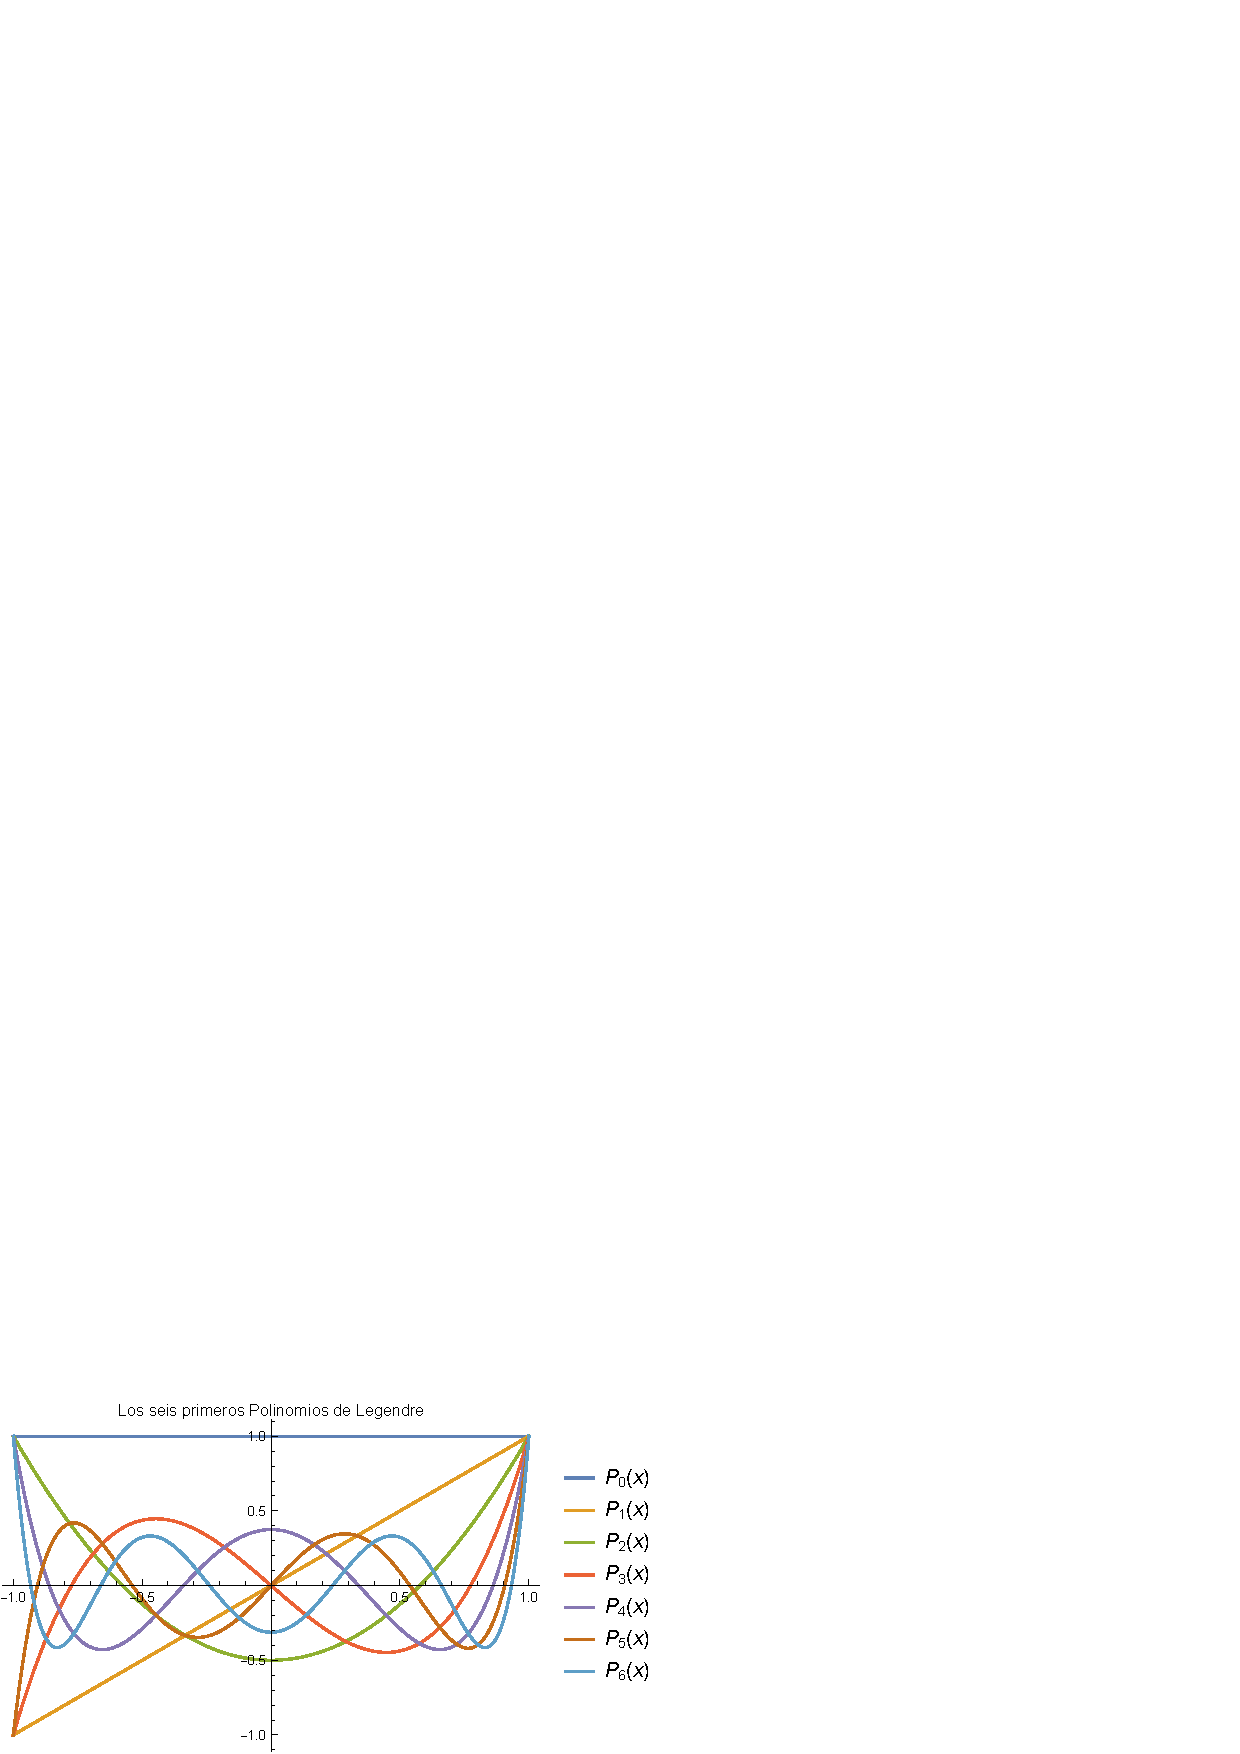
\includegraphics[scale=0.7]{Imagenes/Plot_Lagrange_0-6.pdf}
\end{figure}
\end{frame}
\begin{frame}
\frametitle{Las soluciones}
A pesar de que si $\ell$ es un entero par o impar, respectivamente para $y_{1} (x)$ - ec. (\ref{eq:ecuacion_18_03}) - o $y_{2} (x)$ - ec. (\ref{eq:ecuacion_18_04}), \pause se termina dando un múltiplo del correspondiente polinomio de Legendre $P_{\ell} (x)$, \pause la otra serie en cada caso no termina y por tanto converge sólo para $\abs{x} < 1$.
\end{frame}
\begin{frame}
\frametitle{La segunda solución}
De acuerdo si $\ell$ es par o impar, \pause se definen las \textocolor{ceruleanblue}{funciones de Legendre de segunda clase} como:
\pause
\begin{align*}
Q_{\ell} (x) &=  \alpha_{\ell} \, y_{2} (x) \\
Q_{\ell} (x) &= \beta_{\ell} \, y_{1}(x)
\end{align*}
respectivamente..
\end{frame}
\begin{frame}
\frametitle{La segunda solución}
Donde las constantes $\alpha_{\ell}$ y $\beta_{\ell}$ toman los valores:
\pause
Para $\ell$ par:
\begin{align}
\alpha_{\ell} &=& \dfrac{(-1)^{\ell/2} \; 2^{\ell} \; [(\ell / 2)!]^{2}}{\ell!} \hspace{3.5cm}  \label{eq:ecuacion_18_05}
\end{align}
\pause
Para $\ell$ impar:
\begin{align}
\beta_{\ell} &=& \dfrac{(-1)^{(\ell + 1)/2} \; 2^{\ell - 1} \; \lbrace \left[ (\ell - 1) /2 \right] ! \rbrace^{2}}{\ell!} \label{eq:ecuacion_18_06}
\end{align}
\end{frame}
\begin{frame}
\frametitle{Normalización de las $Q_{\ell} (x)$}
La normalización de los factores se elige de tal manera que $Q_{\ell} (x)$ obedece la misma relación de recurrencia de $P_{\ell}(x)$.
\end{frame}
\begin{frame}
\frametitle{Solución general}
La solución general para la ecuación de Legendre para enteros $\ell$ es por tanto:
\pause
\begin{align}
y (x) = c_{1} \, P_{\ell} (x) + c_{2} \, Q_{\ell} (x) 
\label{eq:ecuacion_18_07}
\end{align}
Donde $P_{\ell} (x)$ es un polinomio de orden $\ell$, que converge para cualquier $x$, y $Q_{\ell} (x)$ es una serie infinita que converge sólo si $\abs{x} < 1$.
\end{frame}
\begin{frame}
\frametitle{Forma cerrada para los $Q_{\ell} (x)$}
Usando el método del Wronkisano, podemos obtener una forma cerrada para $Q_{\ell} (x)$: \pause una segunda solución para la ecuación de Legendre, con $\ell = 0$ es:
\end{frame}
\begin{frame}
\frametitle{Forma cerrada para los $Q_{\ell} (x)$}
\begin{eqnarray}
\begin{aligned}
y_{2}(x) &= P_{0}(x) \scaleint{6ex}^{x} \dfrac{1}{[P_{0}(u)]^{2}} \exp \left( \scaleint{6ex}^{u} \dfrac{2v}{1-v^{2}} \dd{v} \right) \dd{u} = \\ \pause
&= \scaleint{6ex}^{x} \exp [ - \ln (1 - u^{2}) ] \dd{u} = \\ \pause
&= \scaleint{6ex}^{x} \dfrac{du}{(1-u^{2})} = \frac{1}{2} \ln \left( \dfrac{1+x}{1-x} \right)
\end{aligned}
\label{eq:ecuacion_008}
\end{eqnarray}
\pause
En la segunda línea hemos utilizado el hecho de que $P_{0} (x) = 1$.
\end{frame}
\begin{frame}
\frametitle{Ajustando la expresión}
Lo que queda es ajustar la normalización de esta solución para que se corresponda con la ecuación (\ref{eq:ecuacion_18_05}).
\\
\bigskip
\pause
Expandiendo el logaritmo en la ec. (\ref{eq:ecuacion_008}) como una serie de Maclaurin, obtenemos:
\end{frame}
\begin{frame}
\frametitle{Expandiendo el logaritmo}
\begin{align*}
y_{2} (x) = x + \dfrac{x^{3}}{3} + \dfrac{x^{5}}{5} + \cdots
\end{align*}
\pause
Comparando esto con la expresión para $Q_{0} (x)$, usando la ec. (\ref{eq:ecuacion_18_04}) con $\ell = 0$ y normalizando -ec. (\ref{eq:ecuacion_18_05})-, encontramos que $y_{2}$ está correctamente normalizada.
\end{frame}
\begin{frame}
\frametitle{Función normalizada}
Así:
\pause
\begin{align*}
Q_{0} (x) = \dfrac{1}{2} \ln \left( \dfrac{1 + x}{1 - x} \right)
\end{align*}
\end{frame}
\begin{frame}
\frametitle{Función normalizada}
Usando el mismo método para $\ell = 1$, tenemos que:
\pause
\begin{align*}
Q_{1} (x) =  \frac{1}{2} x \ln \left( \dfrac{1 + x}{1 - x} \right) - 1
\end{align*}
\pause
Se pueden encontrar formas cerradas para $Q_{\ell} (x)$ de mayor orden, usando la relación de recurrencia:
\pause
\begin{align*}
(n + 1) \, P_{n+1} = (2 n + 1) \, x \, P_{n} - n \, P_{n-1}
\end{align*}
\end{frame}
\begin{frame}[plain]
\begin{figure}
    \centering
    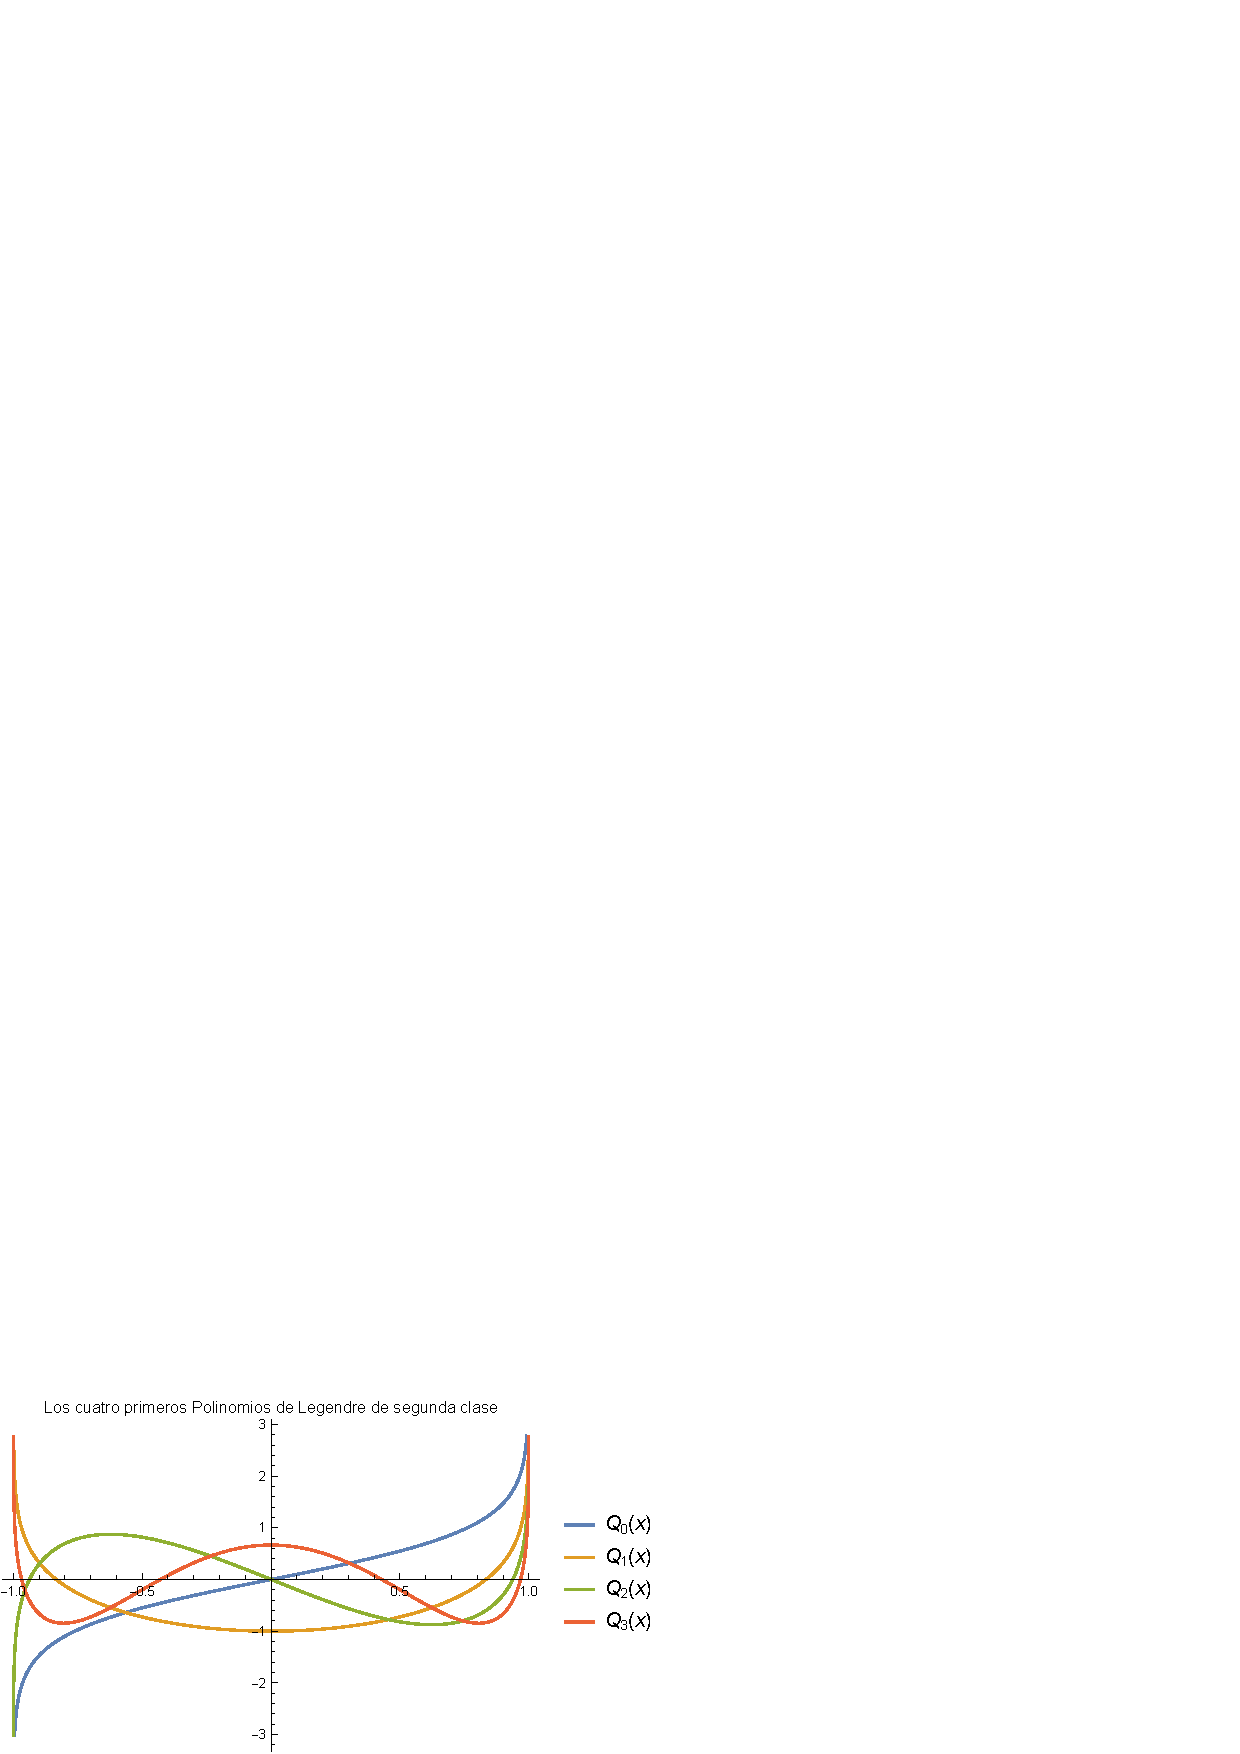
\includegraphics[scale=0.7]{Imagenes/Plot_LagrangeSC_0-4.pdf}
\end{figure}
\end{frame}
  
\section{Propiedades de Legendre}
\frame{\tableofcontents[currentsection, hideothersubsections]}

\begin{frame}
\frametitle{Para problemas físicos}
Como se mencionó anteriormente, cuando encontramos problemas físicos en donde la variable $x$ en la ecuación de Legendre es el coseno del ángulo polar $\theta$ en coordenadas esféricas, \pause y entonces se requiere que la solución $y (x)$ que sea regular en $x = \pm 1$, que corresponde a $\theta = 0$ o $\theta = \pi$. 
\end{frame}
\begin{frame}
\frametitle{Solución como polinomio}
Para que esto ocurra, requerimos que la ecuación tenga una solución polinomial, así el valor de $\ell$ debe ser un entero.
\end{frame}
\begin{frame}
\frametitle{Solución en términos de $P_{\ell} (x)$}
Por otra parte, también requerimos que el coeficiente $c_{2}$ de la función $Q_{\ell}(x)$ en la ecuación (\ref{eq:ecuacion_18_07}) sea nulo, ya que $Q_{\ell}(x)$ es singular en $x = \pm 1$, \pause como resultado de que la solución general es un múltiplo del polinomio de Legendre $P_{\ell} (x)$.
\end{frame}

\subsection{Fórmula de Rodrigues}

\begin{frame}
\frametitle{La expresión}
Como una ayuda para definir nuevas propiedades de los polinomios de Legendre, desarrollamos la representación de Rodrigues de éstas funciones.
\end{frame}
\begin{frame}
\frametitle{La expresión}
La \textocolor{darklava}{fórmula de Rodrigues} para el $P_{\ell} (x)$ es:
\pause
\begin{align}
P_{\ell} (x) = \dfrac{1}{2^{\ell} \; \ell !} \, \dv[\ell]{x}  (x^{2} - 1)^{\ell}
\label{eq:ecuacion_18_09}
\end{align}
\end{frame}

\subsection{Ortogonalidad}

\begin{frame}
\frametitle{ED de tipo Sturm-Liouville}
Del Tema 3, vemos que la ecuación de Legendre es de la forma Sturm-Liouville con:
\pause
\begin{eqnarray*}
\begin{aligned}
p &= 1 - x^{2} \\ \pause
q &= 0 \\ \pause
\lambda &= \ell (\ell + 1) \\ \pause
\omega &= 1
\end{aligned}
\end{eqnarray*}
y que su intervalo natural es $[-1, 1 ]$.
\end{frame}
\begin{frame}
\frametitle{Condición de ortogonalidad}  
Ya que los polinomios de Legendre $P_{\ell} (x)$ son regulares en los puntos extremos $x = \pm 1$, \pause deben ser mutuamente ortogonales en este intervalo, es decir:
\pause
\begin{equation}
\scaleint{6ex}_{-1}^{1} P_{\ell} (x) \, P_{k} (x) \dd{x} = 0 \hspace{1cm} \text{si } \ell \neq k
\label{eq:ecuacion_18_12}
\end{equation}
\end{frame}
\begin{frame}
\frametitle{Expansión de funciones}  
Como ya se comentó previamente, la ortogonalidad mutua (y completes) de $P_{\ell} (x)$ significa que cualquier función razonable $f (x)$ (es decir, una que satisfaga las condiciones de Dirichlet) puede expresarse en el intervalo de $\abs{x} <1$ como una suma infinita de polinomios de Legendre:
\end{frame}
\begin{frame}
\frametitle{Expansión de funciones}
\begin{equation}
f (x) = \nsum_{\ell = 0}^{\infty} a_{\ell} \, P_{\ell} (x)
\label{eq:ecuacion_18_13}
\end{equation}
donde los coeficientes $a_{\ell}$ están dados por:
\pause
\begin{equation}
a_{\ell} = \dfrac{2 \, \ell + 1}{2} \, \scaleint{6ex}_{-1}^{1} f (x) \, P_{\ell} (x) \dd{x}
\label{eq:ecuacion_18_14}
\end{equation}
\end{frame}

\subsection{Función generatriz}

\begin{frame}
\frametitle{De la función generatriz}
Una manera útil para manipular y estudiar las secuencias de funciones o cantidades etiquetadas por una variable entera (en el caso de los polinomios de Legendre $P_{\ell} (x)$ están etiquetados por $\ell$), es mediante una función generatriz. 
\end{frame}
\begin{frame}
\frametitle{De la función generatriz}
La función generatriz tiene quizás su mayor utilidad en el ámbito de la teoría de la probabilidad, sin embargo, también es de gran conveniencia en nuestro estudio.
\end{frame}
\begin{frame}
\frametitle{De la función generatriz}
La función generatriz para decirlo, es una serie de funciones $f_{n} (x)$ para $n = 0, 1, 2,\ldots$, es una función $G (x, h)$ que contiene tanto a $x$, como una variable ficticia $h$, de tal manera que:
\pause
\begin{align*}
G (x, h) = \nsum_{n=0}^{\infty} f_{n} (x) \, h^{n}
\end{align*}
\pause
es decir, $f_{n} (x)$ es el coeficiente de $h^{n}$ en la expansión de $G$ en potencias de $h$.
\end{frame}
\begin{frame}
\frametitle{De la función generatriz}
La utilidad de esta manera de trabajar la función, está en el hecho de que a veces es posible encontrar una forma cerrada para $G (x, h)$.
\end{frame}
\begin{frame}
\frametitle{De la función generatriz}
En el caso de los polinomios de Legendre, usemos las funciones $P_{n} (x)$ definidas por:
\pause
\begin{equation}
G (x, h) = (1 - 2 \, x \, h + h^{2})^{-1/2} =  \nsum_{n=0}^{\infty} P_{n} (x) \, h^{n}
\label{eq:ecuacion_18_15}
\end{equation}
\end{frame}
\begin{frame}
\frametitle{De la función generatriz}
Como veremos las funciones así definidas son idénticas a los polinomios de Legendre y la función $(1 - 2 \, x \, h + h^{2})^{-1/2}$ es de hecho la función generatriz para ellos.
\\
\bigskip
\pause
En el proceso también vamos a deducir varias relaciones útiles entre los diferentes polinomios y sus derivadas.
\end{frame}
\begin{frame}
\frametitle{De la función generatriz}
Hacemos la anotación de que $\dv*{P_{n}(x)}{x}$ es $\pderivada{P} n$, \pause derivamos la ecuación (\ref{eq:ecuacion_18_15}) con respecto a $x$ y obtenemos:
\pause
\begin{equation}
h (1 - 2 \, x \, h + h^{2})^{-3/2} = \nsum \pderivada{P}_{n} \; h^{n}
\label{eq:ecuacion_18_16}
\end{equation}
\end{frame}
\begin{frame}
\frametitle{De la función generatriz}
También derivamos la ecuación (\ref{eq:ecuacion_18_15}) con respecto a $h$ por lo que:
\pause
\begin{equation}
(x - h) (1 - 2 \, x \, h + h^{2})^{-3/2} = \nsum n \; P_{n} \; h^{n-1}
\label{eq:ecuacion_18_17}
\end{equation}
\end{frame}
\begin{frame}
\frametitle{Obteniendo otras relaciones}
La ecuación (\ref{eq:ecuacion_18_16}) puede reescribirse usando la ecuación (\ref{eq:ecuacion_18_15}) como:
\pause
\begin{align*}
h \nsum P_{n} \; h^{n} =  (1 - 2 \, x \, h + h^{2}) \nsum \pderivada{P}_{n} \, h^{n}
\end{align*}
\pause
igualando los coeficientes de $h^{n+1}$, obtenemos la relación de recurrencia:
\pause
\begin{equation}
P_{n} = \pderivada{P}_{n+1} - 2 \, x \; \pderivada{P}_{n} + \pderivada{P}_{n-1}
\label{eq:ecuacion_18_18}
\end{equation}
\end{frame}
\begin{frame}
\frametitle{Obteniendo otras relaciones}
Las ecuaciones (\ref{eq:ecuacion_18_16}) y (\ref{eq:ecuacion_18_17}) pueden combinarse como:
\pause
\begin{align*}
(x - h) \nsum \pderivada{P}_{n} \; h^{n} = h \, \nsum n \; P_{n} \; h^{n-1}
\end{align*}
\end{frame}
\begin{frame}
\frametitle{Obteniendo otras relaciones}
Donde el coeficiente de $h^{n}$ nos proporciona otra relación de recurrencia:
\pause
\begin{equation}
x \pderivada{P}_{n} - \pderivada{P}_{n-1} =  n \; P_{n}
\label{eq:ecuacion_18_19}
\end{equation}
\end{frame}
\begin{frame}
\frametitle{Obteniendo otras relaciones}
Eliminando $\pderivada{P}_{n-1}$ entre las ecuaciones (\ref{eq:ecuacion_18_18}) y (\ref{eq:ecuacion_18_19}), el resulta que se obtiene es:
\pause
\begin{equation}
(n + 1) \, P_{n} = \pderivada{P}_{n+1} - x \; \pderivada{P}_{n}
\label{eq:ecuacion_18_20}
\end{equation}
\end{frame}
\begin{frame}
\frametitle{Obteniendo otras relaciones}
Si tomamos el resultado de la ecuación (\ref{eq:ecuacion_18_20}) re-emplazando $n$ por $n-1$ y sumamos $x$ veces, obtenemos:
\pause
\begin{equation}
(1 - x^{2}) \pderivada{P}_{n} = n \; (P_{n-1} - x P_{n})
\label{eq:ecuacion_18_21}
\end{equation}
\end{frame}
\begin{frame}
\frametitle{Obteniendo otras relaciones}
Finalmente, derivamos ambos lados con respecto a $x$ y usamos el resultado de la ecuación (\ref{eq:ecuacion_18_19}) para tener:
\begin{eqnarray*}
\begin{aligned}
(1 - x^{2}) \sderivada{P}_{n} - 2 \, x \pderivada{P}_{n} &=  n \big[ (\pderivada{P}_{n-1} - x \pderivada{P}_{n}) - P_{n} \big] = \\ \pause
&= n (-n P_{n} - P_{n}) \\ \pause
&= -n (n+1) P_{n}
\end{aligned}
\end{eqnarray*}
\end{frame}
\begin{frame}
\frametitle{Resultado interesante}
El ejemplo anterior muestra que las funciones $P_{n} (x)$ definidas por la ecuación (\ref{eq:ecuacion_18_15}) satisfacen la ecuación de Legendre con $\ell = n$ (un entero) y también de (\ref{eq:ecuacion_18_15}), estas funciones son regulares en $x = \pm 1$.
\end{frame}
\begin{frame}
\frametitle{Resultado interesante}
Entonces $P_{n}$ debe ser un múltiplo del n-ésimo polinomio de Legendre.
\\
\bigskip
\pause
Por lo tanto, sólo queda verificar la normalización.
\end{frame}
\begin{frame}
\frametitle{Normalizando}
Esto se hace fácilmente en $x = 1$, cuando $G$ se convierte en:
\pause
\begin{align*}
G (1, h) = [(1 - h)^{2}]^{-1/2} =  1 + h + h^{2} + \cdots
\end{align*}
\pause
y podemos ver que todo $P_{n}$ así definido, implica que $P_{n} (1) = 1$ como se requiere, \pause por tanto son idénticos a los polinomios de Legendre.
\end{frame}
\begin{frame}
\frametitle{Usando la función generatriz}
Un uso particular de la función generatriz (\ref{eq:ecuacion_18_15}) es la representación del inverso de la distancia entre dos puntos en el espacio tridimensional en términos de polinomios de Legendre.
\end{frame}
\begin{frame}
\frametitle{Usando la función generatriz}
Si dos puntos $\vb{r}$ y $\vb{r}^{\prime}$ se encuentran a distancias $r$ y $\pderivada{r}$, respectivamente, desde el origen, con $\pderivada{r} < r$, se tiene:
\end{frame}
\begin{frame}
\frametitle{Usando la función generatriz}
\begin{eqnarray}
\begin{aligned}
\dfrac{1}{\abs{\vb{r} - \vb{r}^{\prime}}} &= \dfrac{1}{(r^{2} + r^{\prime \: 2} - 2 \, r \, \pderivada{r} \, \cos \theta)^{1/2}} \\[1em] \pause
&= \dfrac{1}{r [ 1 - 2 (\pderivada{r}/r) \cos \theta + (\pderivada{r}/r)^{2}]^{1/2}} \\[1em] \pause
&= \dfrac{1}{r} \nsum_{\ell = 0}^{\infty} \left( \dfrac{\pderivada{r}}{r} \right)^{\ell} \, P_{\ell} (\cos \theta)
\end{aligned}
\label{eq:ecuacion_18_22}
\end{eqnarray}
donde $\theta$ es el ángulo entre los dos vectores de posición $\vb{r}$ y $\vb{r}^{\prime}$.
\end{frame}
\begin{frame}
\frametitle{Usando la función generatriz}
Si $\pderivada{r} > r$, entonces $r$ y $\pderivada{r}$ deben de intercambiarse en la ecuación (\ref{eq:ecuacion_18_22}) o de lo contrario, la serie no converge.
\end{frame}
\begin{frame}
\frametitle{Usando la función generatriz}
Este resultado puede ser utilizado por ejemplo, \pause para escribir el potencial electrostático en un punto $\vb{r}$ debido a una carga $q$ en el punto $\vb{r}^{\prime}$.
\end{frame}
\begin{frame}
\frametitle{Usando la función generatriz}
Entonces, en el caso $\pderivada{r} < r$, se tiene que:
\pause
\begin{align*}
V (\vb{r}) =  \dfrac{q}{4 \, \pi \, \epsilon_{0} \, r} \nsum_{\ell = 0}^{\infty} \left( \dfrac{\pderivada{r}}{r} \right)^{\ell} \, P_{\ell} (\cos \theta)
\end{align*}
\end{frame}
\begin{frame}
\frametitle{Usando la función generatriz}
Vemos el caso especial cuando la carga está en el origen, y $\pderivada{r} = 0$, entonces el término $\ell = 0$ en la serie es no nulo, y al expresión se reduce a la forma ya conocida:
\pause
\begin{align*}
V (\vb{r}) = \frac{q}{4 \, \pi \, \epsilon_{0} \, r}
\end{align*}
\end{frame}

\subsection*{Relaciones de recurrencia}

\begin{frame}
\frametitle{Expresiones de recurrencia}
En nuestro análisis previo de la función generatriz, derivamos varias relaciones de recurrencia útiles que satisfacen los polinomios de Legendre $P_{n} (x)$.
\end{frame}
\begin{frame}
\frametitle{Expresiones de recurrencia}
En particular, a partir de la función generatriz, podemos obtener las siguientes relaciones de recurrencia:
\pause
\begin{eqnarray*}
\begin{aligned}
P_{n} &= P_{n+1}^{\prime} - 2 \, x \; P_{n}^{\prime} + P_{n-1}^{\prime} \\[1em] \pause
x \, P_{n}^{\prime} - P_{n-1}^{\prime} &=  n \, P_{n} \\[1em] \pause
(n + 1) \, P_{n} &= P_{n+1}^{\prime} - x \, P_{n}^{\prime} \\[1em] \pause
P_{n+1}^{\prime} + P_{n-1}^{\prime} &=  P_{n} + 2 \, x \, P_{n}^{\prime} \\[1em] \pause
(1 - x^{2}) \, P_{n+1}^{\prime} &= n \, (P_{n-1} - x \, P_{n}) \\[1em] \pause
(2 \, n + 1) \, P_{n} &= P_{n+1}^{\prime} - P_{n-1}^{\prime}
\end{aligned}
\end{eqnarray*}
\end{frame}
\begin{frame}
\frametitle{Más expresiones}
 De las ecuaciones (\ref{eq:ecuacion_18_19}) a (\ref{eq:ecuacion_18_21}) tenemos las siguientes relaciones de recurrencia con tres términos:
 \pause
\begin{eqnarray*}
\begin{aligned}
\pderivada{P}_{n+1} &= (n+1) \; P_{n} + x \; \pderivada{P}_{n} \\ \pause
\pderivada{P}_{n-1} &= -n \; P_{n} + x \; \pderivada{P}_{n} \\ \pause
(1 - x^{2}) \pderivada{P}_{n+1} &= n \; (P_{n-1} - x \; P_{n}) \\ \pause
(2n+1) P_{n} &= \pderivada{P}_{n+1} - \pderivada{P}_{n-1}
\end{aligned}
\end{eqnarray*}
\end{frame}

\end{document}